\subsection{Question 13}
Le système téléphonique peut être modéliser de la manière suivante : \\

\begin{figure}[H]
  \centering
  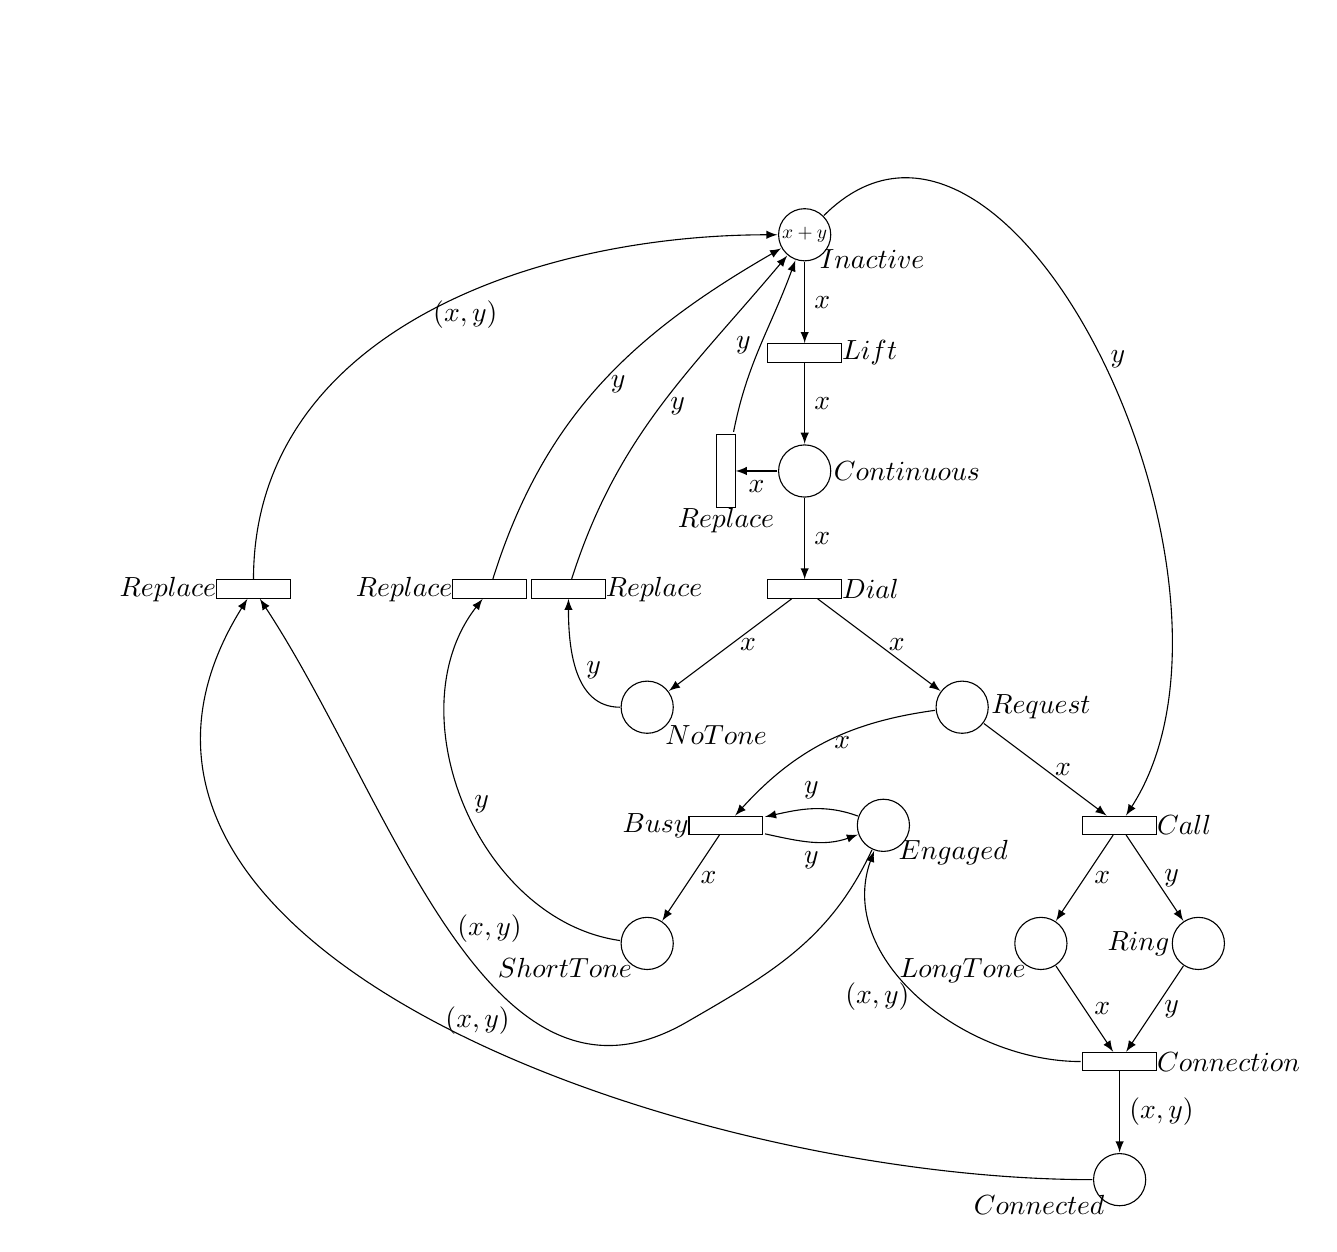
\begin{tikzpicture}
    % Liste des places
    \draw (0,8) node[below right = 2pt] {$Inactive$};
    \node[draw,circle,scale=2] (I) at (0, 8) {};
    \draw (0,5) node[right = 7pt] {$Continuous$};
    \node[draw,circle,scale=2] (C) at (0, 5) {};
    \draw (-2,2) node[below right = 3pt] {$No Tone$};
    \node[draw,circle,scale=2] (NT) at (-2,2) {};
    \draw (2,2) node[right = 7pt] {$Request$};
    \node[draw,circle,scale=2] (Re) at (2, 2) {};
    \draw (1,0.5) node[below right = 2pt] {$Engaged$};
    \node[draw,circle,scale=2] (E) at (1,0.5) {};
    \draw (-2,-1) node[below left = 2pt] {$Short Tone$};
    \node[draw,circle,scale=2] (ST) at (-2, -1) {};
    \draw (3,-1) node[below left = 2pt] {$Long Tone$};
    \node[draw,circle,scale=2] (LT) at (3,-1) {};
    \draw (5,-1) node[left = 7pt] {$Ring$};
    \node[draw,circle,scale=2] (Ri) at (5,-1) {};
    \draw (4,-4) node[below left = 2pt] {$Connected$};
    \node[draw,circle,scale=2] (Co) at (4,-4) {};

  % Liste des transitions
    \draw (0,6.5) node[right = 10pt] {$Lift$};
    \node[draw,rectangle,xscale=4] (L) at (0, 6.5) {};
    \draw (0,3.5) node[right = 10pt] {$Dial$};
    \node[draw,rectangle,xscale=4] (D) at (0, 3.5) {};
    \draw (-1,0.5) node[left = 10pt] {$Busy$};
    \node[draw,rectangle,xscale=4] (B) at (-1, 0.5) {};
    \draw (4,0.5) node[right = 10pt] {$Call$};
    \node[draw,rectangle,xscale=4] (Ca) at (4, 0.5) {};
    \draw (4,-2.5) node[right = 10pt] {$Connection$};
    \node[draw,rectangle,xscale=4] (TCo) at (4, -2.5) {};
    \draw (-1,5) node[below = 10pt] {$Replace$};
    \node[draw,rectangle,yscale=4] (R1) at (-1, 5) {};
    \draw (-3,3.5) node[right = 10pt] {$Replace$};
    \node[draw,rectangle,xscale=4] (R2) at (-3, 3.5) {};
    \draw (-4,3.5) node[left = 10pt] {$Replace$};
    \node[draw,rectangle,xscale=4] (R3) at (-4, 3.5) {};
    \draw (-7,3.5) node[left = 10pt] {$Replace$};
    \node[draw,rectangle,xscale=4] (R4) at (-7, 3.5) {};

  % Liste des arcs
    \draw[->,>=latex] (I) -- (L)node[midway, right]{$x$};
    \draw[->,>=latex] (L) -- (C)node[midway, right]{$x$};
    \draw[->,>=latex] (C) -- (R1)node[midway, below]{$x$};
    \draw[->,>=latex] (C) -- (D)node[midway, right]{$x$};
    \draw[->,>=latex] (D) -- (NT)node[midway, right]{$x$};
    \draw[->,>=latex] (D) -- (Re)node[midway, right]{$x$};
    \draw[->,>=latex] (Re) -- (Ca)node[midway, right]{$x$};
    \draw[->,>=latex] (Re) to[bend right=20] node[midway, right]{$x$} (B);
    \draw[->,>=latex] (Ca) -- (Ri)node[midway, right]{$y$};
    \draw[->,>=latex] (Ca) -- (LT)node[midway, right]{$x$};
    \draw[->,>=latex] (B) -- (ST)node[midway, right]{$x$};
    \draw[->,>=latex] (E) to[out=160, in=20] node[midway, above]{$y$} (B);
    \draw[->,>=latex] (B) to[out=-20,in=200] node[midway, below]{$y$} (E);
    \draw[->,>=latex] (LT) -- (TCo)node[midway, right]{$x$};
    \draw[->,>=latex] (Ri) -- (TCo)node[midway, right]{$y$};
    \draw[->,>=latex] (TCo) -- (Co)node[midway, right]{$(x,y)$};
    \draw[->,>=latex] (I) to[out=45,in=60] node[midway, right]{$y$}(Ca);
    \draw[->,>=latex] (R1) to[out=75,in=-110] node[midway, left]{$y$}(I);
    \draw[->,>=latex] (NT) to[out=180,in=-90] node[midway, right]{$y$}(R2);
    \draw[->,>=latex] (R2) to[out=75,in=-130] node[midway, right]{$y$}(I);
    \draw[->,>=latex] (ST) to[bend left=60] node[midway, right]{$y$}(R3);
    \draw[->,>=latex] (R3) to[out=75,in=-150] node[midway, right]{$y$}(I);
    \draw[->,>=latex] (TCo) to[out=180,in=-110] node[midway, left]{$(x,y)$}(E);
    \draw[->,>=latex] (Co) to[out=180,in=-120] node[midway, right]{$(x,y)$}(R4);
    \draw[->,>=latex] (R4) to[out=90,in=-180] node[midway, right]{$(x,y)$}(I);
    \draw[->,>=latex] (E) to[out=-115,in=30] (-1.5,-2) to[out=210,in=-60]  node[midway, right]{$(x,y)$}(R4);


    %Marquage
    \node(M0)[scale=0.7] at (0,8) {$x+y$};

  \end{tikzpicture}
  \caption{Réseau de petri associé au contrôle d'un système téléphonique} \label{fig:M1}
\end{figure}

\subsection{Question 2}

\begin{enumerate}
\item Evolution du sytème\\
Initialement, on considère que les deux téléphones sont inactifs.\\
on choisit arbitrairement la couleur $x$ pour désigner l'appelant et $y$ l'appelé.\\
Lorsque $x$ décroche sont téléphone(transition $Lift$), il entend une sonnerie continue représentée par la place $Continuous$.\\
À ce moment, $x$ peut soit raccrocher, $replace$, et redevenir inactif, soit composer un numéro, $Dial$ et attendre la réponse à sa demande, $Request$.\\
Si l'appelé $y$ est déjà en communication, $Engaged$, alors on sensibilise la transition $Busy$.\\
$y$ reste dans sa communication, $Engaged$, et $x$ recoit de courte sonnerie, $Short Tone$ avant de raccrocher, $replace$, et devenir inactive.\\
Si l'appelé $y$ est inactif, alors l'appel est envoyé, $Call$, et une longue sonnerie est envoyé à l'appelant, $x$ en $Long Tone$, et on fait sonner le téléphone de l'appelé, $y$ en $Ring$.\\
Lorsque l'appelé décroche, la connection s'établie entre les deux téléphones, $Connection$, et il sont en communication $Connected$.\\
Enfin, quand ils raccrochent, $replace$, ils redeviennent tous deux inactifs.

\item Cas particuliers
  \begin{itemize}
    \item Lorsque qu'un usager s'appele soit même, il va être engager dès qu'il va d'écrocher, donc il aura une sonnerie occupée. 
    \item Dans la modelisation que nous avons fait, la fin de connection peut être initier autant par l'appelant que par l'appelé.
    \item Avec nos maigre connaissance en téléphonie, il nous est difficile de dire avec certitude quel systême est utilisé en france.\\
Mais nous pensons que le modèle que nous avons fait peut correspondre au systême français.

  \end{itemize}
\end{enumerate}

\newpage
